\documentclass[12pt]{article}
\usepackage[T1, T2A]{fontenc}
\usepackage[utf8]{inputenc}
\usepackage[russian]{babel}
\usepackage{hyperref}
\usepackage{datetime}
\usepackage{listings}
\usepackage{amsmath}
\usepackage{amsfonts}
\usepackage{tikz}
\usepackage{multirow}
\graphicspath{ {./Images/} }

% For slope Fields
\usepackage{pgfplots}
\usetikzlibrary{calc}
\usetikzlibrary{shapes.geometric, arrows.meta, positioning}
\pgfplotsset{compat=1.8}

\usepackage[14pt]{extsizes} % для того чтобы задать нестандартный 14-ый размер шрифта
\usepackage[utf8]{inputenc}
\usepackage[russian]{babel} % поддержка русского языка
\usepackage{amsmath}  %  математические символы
\usepackage[left=20mm, top=15mm, right=15mm, bottom=30mm, footskip=15mm]{geometry} % настройки полей документа
\usepackage{indentfirst} % по умалчанию убирается отступ у первого абзаца в секции, это отменяет это.
\usepackage{paralist} % добавить компактные списки (compactitem, compactenum, compactdesc)

\usepackage{fancyvrb}
\usepackage{framed}

\DeclareMathOperator{\cov}{cov}

\begin{document}
% \maketitle
\begin{titlepage}

	\begin{center}
		\hfill \break
		\textbf{
			\large{РОССИЙСКИЙ УНИВЕРСИТЕТ ДРУЖБЫ НАРОДОВ}\\
			\normalsize{Факультет физико-математических и естественных наук}\\
			\normalsize{Кафедра прикладной информатики и теории вероятностей}\\
		}
		\vspace*{\fill}
		\Large{\textbf{Лабораторная работа №3}}
		\\
		\underline{\textit{\normalsize{Дисциплина: Имитационное моделирование}}}
		\vspace*{\fill}

	\end{center}

	\begin{flushright}
		Студент: \underline{Григорий Матюхин}\\ \vspace{0.5cm}
		Группа: \underline{НПИбд-01-21}
	\end{flushright}


	\begin{center} \textbf{МОСКВА} \\ 2023 г. \end{center}
	\thispagestyle{empty} % выключаем отображение номера для этой страницы

\end{titlepage}
\newpage
\tableofcontents
\newpage

\section{Постановка задания}
Морские судна двух типов прибывают в порт, где происходит их разгрузка. В порту есть
два буксира, обеспечивающих ввод кораблей в порт и вывод из порта. К первому типу
судов относятся корабли малого тоннажа, которые требуют использования одного
буксира. Корабли второго типа имеют большие размеры, для их ввода и вывода из порта
требуется два буксира. Из-за различия размеров двух типов кораблей необходимы и
причалы различного размера. Кроме того, корабли имеют различное время погрузки-
разгрузки. Исходные данные приведены в таблице:

\begin{tabular}{|l|c|c|}
	\hline
	\multicolumn{1}{|c|}{\multirow{2}{4em}{Параметр}} & \multicolumn{2}{|c|}{Тип корабля}              \\
	\cline{2-3}
	                                                  & 1                                 & 1          \\
	\hline
	Интервал прибытия, мин.                           & $130\pm30$                        & $390\pm60$ \\
	\hline
	Время входа в порт, мин.                          & $30\pm7$                          & $45\pm12$  \\
	\hline
	Количество причалов                               & 6                                 & 3          \\
	\hline
	Время погрузки-разгрузки, час.                    & $12\pm2$                          & $18\pm4$   \\
	\hline
	Время выхода из порта, мин.                       & $20\pm5$                          & $35\pm10$  \\
	\hline
\end{tabular} \\

Постройте модель системы, в которой можно оценить время ожидания кораблями каждого
типа входа в порт. (Время ожидания входа в порт включает время ожидания
освобождения причала и буксира.) Корабль, ожидающий освобождения причала, не
обслуживается буксиром до тех пор, пока не будет предоставлен нужный причал. Корабль
второго типа не займет буксир до тех пор, пока ему не будут доступны два буксира.

\begin{enumerate}
	\item Проведя расчеты по программе, ответьте на вопросы:
	      \begin{enumerate}
		      \item каково среднее время ожидания кораблями каждого типа входа в порт?
		      \item как изменится среднее время ожидания кораблями каждого типа входа в порт, если
		            количество буксиров увеличить с двух до трех?
	      \end{enumerate}
	\item Выведите на экран график очереди судов второго типа. Существенна ли возникающая
	      очередь?
	\item Предположим, что возросла интенсивность движения судов второго типа: интервал
	      времени прибытия уменьшился с 390 до 240 минут. Можно ли ликвидировать возникшую
	      очередь, если увеличить количество причалов для кораблей второго типа с трех до
	      четырех? С трех до пяти?
\end{enumerate}

\section{Код программы}
\begin{lstlisting}
; Time unit - 1 minute

dock1	STORAGE 6
dock2	STORAGE 3
tugs	STORAGE 2

; Small ships
      GENERATE 130,30
      QUEUE type1
      ENTER dock1
      ENTER tugs
      DEPART type1
      ADVANCE 30,7
      LEAVE tugs
      ADVANCE 720,120	; 12 +- 2 hours
      ENTER tugs
      LEAVE dock1
      ADVANCE 20,5
      LEAVE tugs
      TERMINATE

; Big ships
      GENERATE 390,60
      QUEUE type2
      ENTER dock2
      ENTER tugs,2
      DEPART type2
      ADVANCE 45,12
      LEAVE tugs,2
      ADVANCE 1080,240	; 18 +- 4 hours
      ENTER tugs,2
      LEAVE dock2
      ADVANCE 35,10
      LEAVE tugs,2
      TERMINATE

; Timer
      GENERATE 1000000
      TERMINATE 1

; Control
      START 1
\end{lstlisting}

\section{Ответ}

\begin{enumerate}
	\item \mbox{} \\
	      \begin{enumerate}
		      \item 93.078; 2384.245 ---
		            среднее время ожидания кораблей первого и второго типов, соответственно.
		      \item 54.0.45; 722.990 ---
		            новое среднее время ожидания кораблей первого и второго типов, соответственно.
	      \end{enumerate}
	\item \mbox{} \\
	      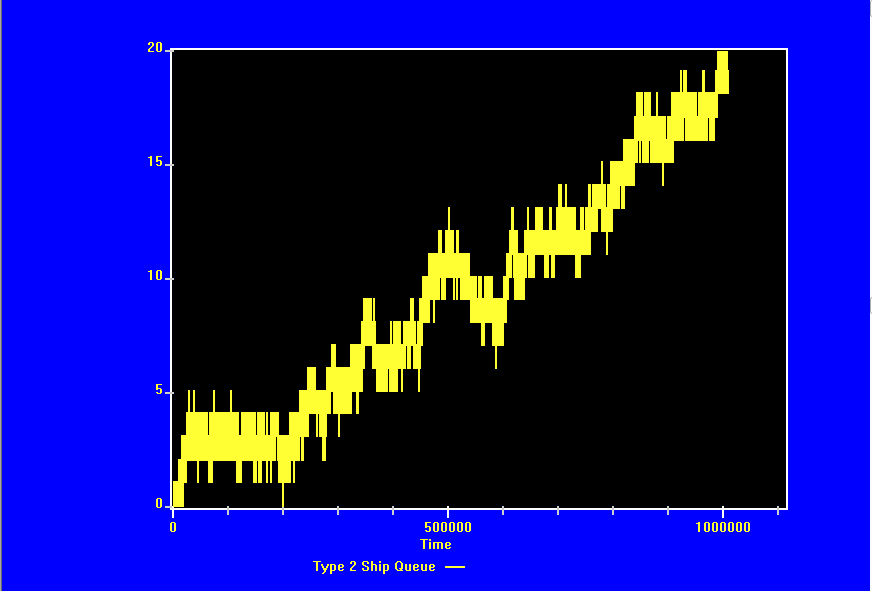
\includegraphics[scale=0.7]{plot.png}
	\item Да, возникшую очередь возможно ликвидировать,
	      если увеличить количество причалов для кораблей второго типа с трех до пяти.

\end{enumerate}

\end{document}
